\section{How does Intel SGX work}

\begin{frame}
    \frametitle{Overview}
    \begin{itemize}
        \visible<1->{\item Application is split into a secure part and a non-secure part}
        \visible<2->{\item Secure part is called \glqq{}enclave\grqq{}}
        \visible<3->{\item Application contains own code, its own data and the enclave}
        \visible<4>{\item Enclave is launched by the application through a call to the encalve entry point}
    \end{itemize}
\end{frame}

\begin{frame}
    \frametitle{Overview}
    \begin{itemize}
        \visible<1->{\item Enclave contains also its own code and data}
        \visible<2->{\item Enclave is safed through encrypted memory pages which are reserved inside the RAM}
        \visible<3->{\item The OS itself can not read data from the enclave, because encryption is oon hardware layer}
        \visible<3->{\item The encrypted memory pages can only be accessed from the enclave, not from the application}
        \visible<4->{\item Enclave entry point is pre-defined during compilation and won't change}
        \visible<5->{\item Enclaves can access their application memory, but not the other way arround}
        \visible<6>{\item An enclave can be called by multiple threads up to the number of logical processors}
    \end{itemize}
\end{frame}

\begin{frame}
    \frametitle{Overview}
    \centering
    \begin{figure}
        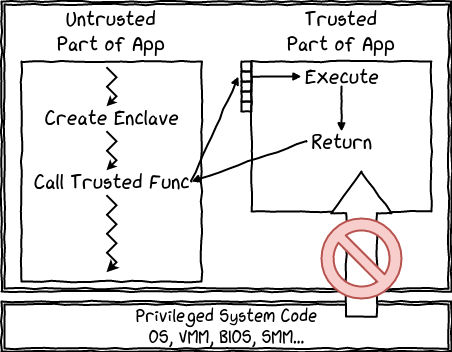
\includegraphics[scale=0.5]{Images/sgx_overview.png}
        \caption{Quelle: \url{https://blog.quarkslab.com/overview-of-intel-sgx-part-1-sgx-internals.html}}
    \end{figure}
\end{frame}

\begin{frame}
    \frametitle{Instructions}
    \begin{itemize}
        \visible<1->{\item Intel SGX defines 18 new Instructions to handle the enclaves}
        \visible<2->{\item These Instructions are systemcalls to handle the enclave}
        \visible<3->{\item Processor need these new instructions, because the enclave is on the hardware layer}
        \visible<4->{\item All instructions are implemented in mircro-code, so that the behaviour can be modified}
        \visible<5-> {\item 13 instructions can be used by the supervisor which is the kernel mode}
        \visible<6->{\item 5 instructions can e used by normal users}
        \visible<7->{\item Example for Instructions are EENTRY or EEXIT}
        \visible<8>{\item The processor can enter or exit the enclave with this two instructions}
    \end{itemize}
\end{frame}

\begin{frame}
    \frametitle{Structures}
    \begin{itemize}
        \visible<1->{\item Intel SGX defines 13 new structures which are used to manage the enclave and the associated data}
        \visible<2->{\item These structures are like a library for the processor and the enclaves}
        \visible<2->{\item 8 structures are used for enclave managment}
        \visible<3->{\item 3 structures are used for memory page managment}
        \visible<4->{\item 2 structures are used for resources managment}
        \visible<5>{\item SGX enclave control structure (SECS) contains meta-data like hash value or the enclave size}
    \end{itemize}
\end{frame}

\begin{frame}
    \frametitle{Enclave Page Cache (EPC)}
    \begin{itemize}
        \visible<1->{\item Code and data of the enclave is stored in a special memory area, called EPC}
        \visible<2->{\item This area is encrypted by using the Memory Encryption Engine (MME)}
        \visible<3->{\item MME is an extra new and dedicated chip for Intel SGX}
        \visible<4->{\item External reads can only observe encrypted data outside the chip}
        \visible<5->{\item The pages are only decrypted when read is inside the physical processor core}
        \visible<6>{\item Keys for decrypting are generated at boot-time and are stored inside the CPU}
    \end{itemize}
\end{frame}

\begin{frame}
    \frametitle{Page Check}
    \begin{itemize}
        \visible<1->{\item Page check is extended to prevent external access to EPC}
        \visible<2->{\item The Enclave Page Cache Map (EPCM) is one of the 13 structures}
        \visible<3->{\item EPCM is used to store the pages state and contains the configuration, permissions and type of each page}
        \visible<4>{\item EPCM is also stored inside the protected memory area and grants access to the page}
    \end{itemize}
\end{frame}

\begin{frame}
    \frametitle{Page Check}
    \centering
    \begin{figure}
        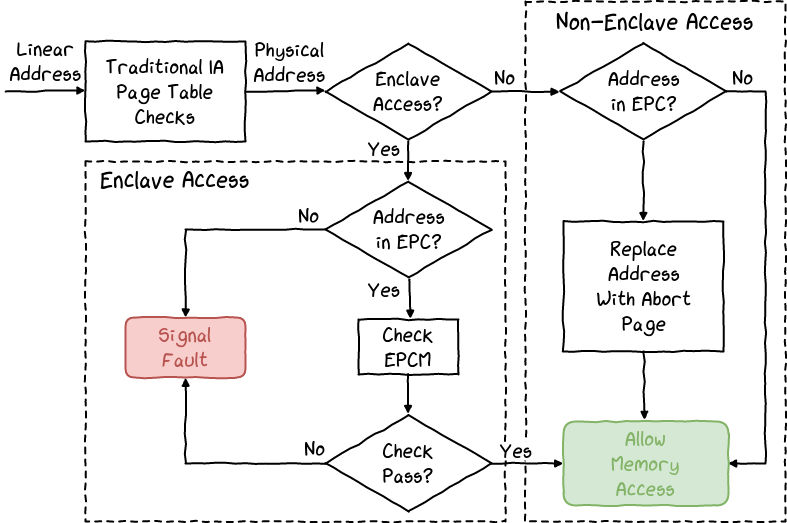
\includegraphics[scale=0.35]{Images/epc_pageCheck.png}
        \caption{Quelle: \url{https://blog.quarkslab.com/overview-of-intel-sgx-part-1-sgx-internals.html}}
    \end{figure}
\end{frame}

\begin{frame}
    \frametitle{procedure application with enclave}
    \begin{columns}
        \begin{column}{0.3\textwidth}
           \begin{enumerate}
               \visible<1->{\item EENTRY instruction is executed to enter enclave}
               \visible<2->{\item The application context is saved}
               \visible<3->{\item The processor is put in enclave mode}
               \visible<4->{\item EEXIT instruction is executed to exit enclave}
               \visible<5>{\item The processor is put in normal mode}
           \end{enumerate}
        \end{column}
        \begin{column}{0.7\textwidth}
            \begin{center}
                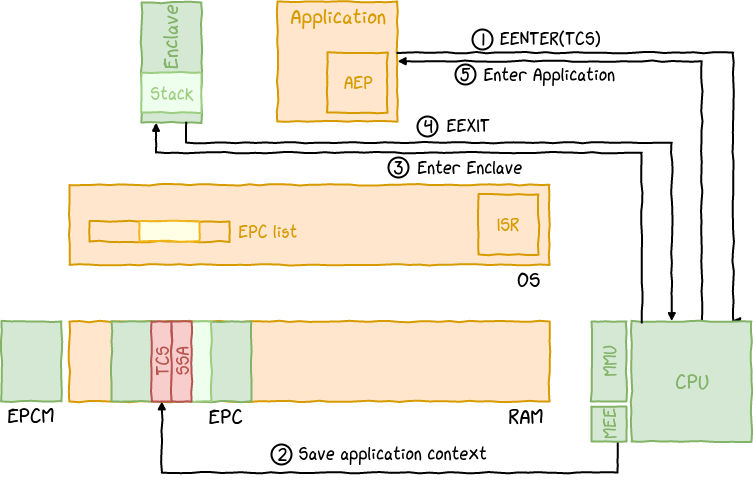
\includegraphics[scale=0.35]{Images/procedure.png}
            \end{center}
        \end{column}
        \end{columns}
\end{frame}

\begin{frame}
    \frametitle{Local Attestation}
    \begin{itemize}
        \visible<1->{\item Enclaves can communicate to each other}
        \visible<2->{\item Local attestation is a proof, that the otzer enclave exists and is trustable}
        A channel must have been established between the two enclaves
    \end{itemize}
\end{frame}

\begin{frame}
    \frametitle{Local Attestation}
    \begin{enumerate}
        \visible<1->{\item The first enclave can ask the hardware to generate a credential, named report, and send it to the other enclave}
        \visible<2->{\item The second can verify, that this resport is generated on the same platform and can now trust this enclave}
        \visible<3>{\item The second enclave has also to proof the report of the first enclave}
    \end{enumerate}
\end{frame}

%vielleicht mit Bild als erklärung leichter????????

\begin{frame}
    \frametitle{Remote Attestation}
    \begin{itemize}
        \visible<1->{\item Remote attestation is an exchange of a \glqq{}quote\grqq{}}
        \visible<2->{\item Remote attestation needs an extra architectural enclave, called \glqq{}quoting enclave\grqq{}}
        \visible<3->{\item This extra enclave is an architectural enclave, called \glqq{}quoting enclave\grqq{}}
        \visible<4->{\item The quoting enclave verifies and transforms the enclave report into a quote}
        \visible<5->{\item A quote is signed by the quoting enclave by the Provisioning Key}
        \visible<6>{\item This quote is remotely verifiable}
    \end{itemize}
\end{frame}

\begin{frame}
    \frametitle{Remote Attestation}
    \begin{enumerate}
        \visible<1->{\item An attestation request is send from a server to the application}
        \visible<2->{\item The application sends a report request to the application enclave}
        \visible<3->{\item The application enclave returns the generated report}
        \visible<4->{\item The application receives the report and forwards it to the quoting enclave to be signed}
        \visible<5->{\item The quoting enclave generates from the report a quote and the quote is send back to the application}
        \visible<6->{\item The application sends the quote to the server for verification}
        \visible<7->{\item The server validates the quote signature and the server sends the data to the attestation service}
    \end{enumerate}
\end{frame}

%vielleicht mit Bild als erklärung leichter????????

\begin{frame}
    \frametitle{Sealing}
    \begin{itemize}
        \visible<1->{\item Process of encrypting enclave secrets for persistent sorage is calles sealing}
        \visible<2->{\item Different ways of sealing}
        \visible<3->{\item Enclave retrieves the seal Key using the EGETKEY instruction, which returns a cryptographical key}
        \visible<4>{\item Key is used to encrypt and ensure data integrity}
    \end{itemize}
\end{frame}

\begin{frame}
    \frametitle{Sealing - Different ways}
    \begin{itemize}
        \visible<1->{\item Enclave Identity}
        \visible<2->{\begin{itemize}
            \item Two distinct enclaves have different keys
            \item Sealed data will not be available to different versions of the same enclave
            \item Sealed data will only be available to identical enclave instantiations
        \end{itemize}}
        \visible<3->{\item Signer Identity}
        \visible<4->{\begin{itemize}
            \item Two distinct enclaves have different keys
            \item Two versions of an enclave share the same key
            \item multiple enclaves which are using the same key can all read each others data
        \end{itemize}}
        \visible<5->{\item Security Version Number (SVN)}
        \visible<6>{\begin{itemize}
            \item SVN is a counter which is incremented after each update
            \item Older versions of an enclave are not available to read data from a newer version
            \item keys are derived that an enclave can retrieve the keys corresponding to current or older security level
        \end{itemize}}
    \end{itemize}

    

\end{frame}

